%
%    Generated: VHDL to LaTeX
%    URL:       www.mamikon.net
%    Author:    Anna Bansaghi
%    Version:   1.0.5
%    Date:      4 December 2016
%
\documentclass{standalone}
\usepackage{tikz}
\usetikzlibrary{calc,arrows}
\makeatletter
\pgfdeclareshape{circuit}{
  \savedanchor\northeast{
    \pgfmathsetlength\pgf@x{\pgfshapeminwidth}
    \pgfmathsetlength\pgf@y{\pgfshapeminheight}
    \pgf@x=0.7\pgf@x
    \pgf@y=0.5\pgf@y}
  \savedanchor\southwest{
    \pgfmathsetlength\pgf@x{\pgfshapeminwidth}
    \pgfmathsetlength\pgf@y{\pgfshapeminheight}
    \pgf@x=-0.7\pgf@x
    \pgf@y=-1.15\pgf@y}
  \inheritanchorborder[from=rectangle]
  \anchor{center}{\pgfpointorigin}
  \anchor{north}{\northeast \pgf@x=0pt}
  \anchor{east}{\northeast \pgf@y=0pt}
  \anchor{south}{\southwest \pgf@x=0pt}
  \anchor{west}{\southwest \pgf@y=0pt}
  \anchor{north east}{\northeast}
  \anchor{north west}{\northeast \pgf@x=-\pgf@x}
  \anchor{south west}{\southwest}
  \anchor{south east}{\southwest \pgf@x=-\pgf@x}
  \anchor{text}{
    \pgfpointorigin
    \advance\pgf@x by -.5\wd\pgfnodeparttextbox
    \advance\pgf@y by -3.8625\ht\pgfnodeparttextbox
    \advance\pgf@y by +.5\dp\pgfnodeparttextbox}
\anchor{ina}{
  \pgf@process{\northeast}
  \pgf@x=-1\pgf@x
  \pgf@y=0.5\pgf@y}
\anchor{inb}{
  \pgf@process{\northeast}
  \pgf@x=-1\pgf@x
  \pgf@y=0.09999999999999998\pgf@y}
\anchor{inc}{
  \pgf@process{\northeast}
  \pgf@x=-1\pgf@x
  \pgf@y=-0.6000000000000001\pgf@y}
\anchor{ind}{
  \pgf@process{\northeast}
  \pgf@x=-1\pgf@x
  \pgf@y=-1\pgf@y}
\anchor{ine}{
  \pgf@process{\northeast}
  \pgf@x=-1\pgf@x
  \pgf@y=-1.4\pgf@y}
\anchor{inf}{
  \pgf@process{\northeast}
  \pgf@x=-1\pgf@x
  \pgf@y=-1.8\pgf@y}
\anchor{outa}{
  \pgf@process{\northeast}
  \pgf@y=0.5\pgf@y}
\anchor{outb}{
  \pgf@process{\northeast}
  \pgf@y=0.09999999999999998\pgf@y}
\anchor{outc}{
  \pgf@process{\northeast}
  \pgf@y=-0.3\pgf@y}
\anchor{outd}{
  \pgf@process{\northeast}
  \pgf@y=-0.7000000000000001\pgf@y}
\backgroundpath{
  \pgfpathrectanglecorners{\southwest}{\northeast}
  \begingroup
    \tikzset{labels}
    \tikz@textfont
  \endgroup}}
\tikzset{add font/.code={\expandafter\def\expandafter\tikz@textfont\expandafter{\tikz@textfont#1}}}
\tikzset{labels/.style={font=\sffamily\scriptsize}}
\tikzset{every circuit node/.style={draw,minimum width=2cm,minimum height=2.5cm,very thick,inner sep=1mm,outer sep=0pt,cap=round,add font=\sffamily\bfseries}}
\makeatother
\begin{document}
\centering
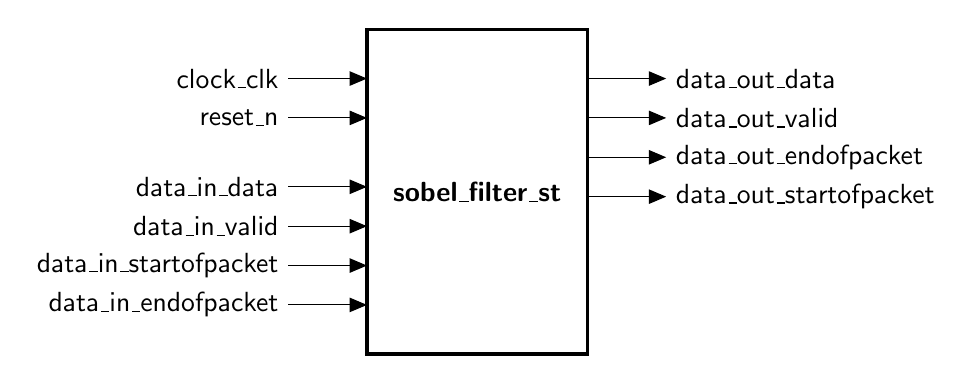
\begin{tikzpicture}[font=\sffamily,>=triangle 45]
  \node [shape=circuit] (item) at (0,0) {sobel\_filter\_st};
  \draw [<-] (item.ina) node [anchor=west,labels] {} -- +(-1,0) node [anchor=east] {clock\_clk};
  \draw [<-] (item.inb) node [anchor=west,labels] {} -- +(-1,0) node [anchor=east] {reset\_n};
  \draw [<-] (item.inc) node [anchor=west,labels] {} -- +(-1,0) node [anchor=east] {data\_in\_data};
  \draw [<-] (item.ind) node [anchor=west,labels] {} -- +(-1,0) node [anchor=east] {data\_in\_valid};
  \draw [<-] (item.ine) node [anchor=west,labels] {} -- +(-1,0) node [anchor=east] {data\_in\_startofpacket};
  \draw [<-] (item.inf) node [anchor=west,labels] {} -- +(-1,0) node [anchor=east] {data\_in\_endofpacket};
  \draw [->] (item.outa) node [anchor=east,labels] {} -- +(1,0) node [anchor=west] {data\_out\_data};
  \draw [->] (item.outb) node [anchor=east,labels] {} -- +(1,0) node [anchor=west] {data\_out\_valid};
  \draw [->] (item.outc) node [anchor=east,labels] {} -- +(1,0) node [anchor=west] {data\_out\_endofpacket};
  \draw [->] (item.outd) node [anchor=east,labels] {} -- +(1,0) node [anchor=west] {data\_out\_startofpacket};
\end{tikzpicture}
\end{document}
